% Options for packages loaded elsewhere
\PassOptionsToPackage{unicode}{hyperref}
\PassOptionsToPackage{hyphens}{url}
%
\documentclass[
  ignorenonframetext,
]{beamer}
\usepackage{pgfpages}
\setbeamertemplate{caption}[numbered]
\setbeamertemplate{caption label separator}{: }
\setbeamercolor{caption name}{fg=normal text.fg}
\beamertemplatenavigationsymbolsempty
% Prevent slide breaks in the middle of a paragraph
\widowpenalties 1 10000
\raggedbottom
\setbeamertemplate{part page}{
  \centering
  \begin{beamercolorbox}[sep=16pt,center]{part title}
    \usebeamerfont{part title}\insertpart\par
  \end{beamercolorbox}
}
\setbeamertemplate{section page}{
  \centering
  \begin{beamercolorbox}[sep=12pt,center]{part title}
    \usebeamerfont{section title}\insertsection\par
  \end{beamercolorbox}
}
\setbeamertemplate{subsection page}{
  \centering
  \begin{beamercolorbox}[sep=8pt,center]{part title}
    \usebeamerfont{subsection title}\insertsubsection\par
  \end{beamercolorbox}
}
\AtBeginPart{
  \frame{\partpage}
}
\AtBeginSection{
  \ifbibliography
  \else
    \frame{\sectionpage}
  \fi
}
\AtBeginSubsection{
  \frame{\subsectionpage}
}
\usepackage{lmodern}
\usepackage{amssymb,amsmath}
\usepackage{ifxetex,ifluatex}
\ifnum 0\ifxetex 1\fi\ifluatex 1\fi=0 % if pdftex
  \usepackage[T1]{fontenc}
  \usepackage[utf8]{inputenc}
  \usepackage{textcomp} % provide euro and other symbols
\else % if luatex or xetex
  \usepackage{unicode-math}
  \defaultfontfeatures{Scale=MatchLowercase}
  \defaultfontfeatures[\rmfamily]{Ligatures=TeX,Scale=1}
\fi
\usetheme[]{Hannover}
\usecolortheme{dove}
\usefonttheme{structurebold}
% Use upquote if available, for straight quotes in verbatim environments
\IfFileExists{upquote.sty}{\usepackage{upquote}}{}
\IfFileExists{microtype.sty}{% use microtype if available
  \usepackage[]{microtype}
  \UseMicrotypeSet[protrusion]{basicmath} % disable protrusion for tt fonts
}{}
\makeatletter
\@ifundefined{KOMAClassName}{% if non-KOMA class
  \IfFileExists{parskip.sty}{%
    \usepackage{parskip}
  }{% else
    \setlength{\parindent}{0pt}
    \setlength{\parskip}{6pt plus 2pt minus 1pt}}
}{% if KOMA class
  \KOMAoptions{parskip=half}}
\makeatother
\usepackage{xcolor}
\IfFileExists{xurl.sty}{\usepackage{xurl}}{} % add URL line breaks if available
\IfFileExists{bookmark.sty}{\usepackage{bookmark}}{\usepackage{hyperref}}
\hypersetup{
  pdftitle={Session 10: Repeated Measures and Longitudinal Analysis II},
  pdfauthor={Levi Waldron},
  hidelinks,
  pdfcreator={LaTeX via pandoc}}
\urlstyle{same} % disable monospaced font for URLs
\newif\ifbibliography
\usepackage{color}
\usepackage{fancyvrb}
\newcommand{\VerbBar}{|}
\newcommand{\VERB}{\Verb[commandchars=\\\{\}]}
\DefineVerbatimEnvironment{Highlighting}{Verbatim}{commandchars=\\\{\}}
% Add ',fontsize=\small' for more characters per line
\usepackage{framed}
\definecolor{shadecolor}{RGB}{248,248,248}
\newenvironment{Shaded}{\begin{snugshade}}{\end{snugshade}}
\newcommand{\AlertTok}[1]{\textcolor[rgb]{0.94,0.16,0.16}{#1}}
\newcommand{\AnnotationTok}[1]{\textcolor[rgb]{0.56,0.35,0.01}{\textbf{\textit{#1}}}}
\newcommand{\AttributeTok}[1]{\textcolor[rgb]{0.77,0.63,0.00}{#1}}
\newcommand{\BaseNTok}[1]{\textcolor[rgb]{0.00,0.00,0.81}{#1}}
\newcommand{\BuiltInTok}[1]{#1}
\newcommand{\CharTok}[1]{\textcolor[rgb]{0.31,0.60,0.02}{#1}}
\newcommand{\CommentTok}[1]{\textcolor[rgb]{0.56,0.35,0.01}{\textit{#1}}}
\newcommand{\CommentVarTok}[1]{\textcolor[rgb]{0.56,0.35,0.01}{\textbf{\textit{#1}}}}
\newcommand{\ConstantTok}[1]{\textcolor[rgb]{0.00,0.00,0.00}{#1}}
\newcommand{\ControlFlowTok}[1]{\textcolor[rgb]{0.13,0.29,0.53}{\textbf{#1}}}
\newcommand{\DataTypeTok}[1]{\textcolor[rgb]{0.13,0.29,0.53}{#1}}
\newcommand{\DecValTok}[1]{\textcolor[rgb]{0.00,0.00,0.81}{#1}}
\newcommand{\DocumentationTok}[1]{\textcolor[rgb]{0.56,0.35,0.01}{\textbf{\textit{#1}}}}
\newcommand{\ErrorTok}[1]{\textcolor[rgb]{0.64,0.00,0.00}{\textbf{#1}}}
\newcommand{\ExtensionTok}[1]{#1}
\newcommand{\FloatTok}[1]{\textcolor[rgb]{0.00,0.00,0.81}{#1}}
\newcommand{\FunctionTok}[1]{\textcolor[rgb]{0.00,0.00,0.00}{#1}}
\newcommand{\ImportTok}[1]{#1}
\newcommand{\InformationTok}[1]{\textcolor[rgb]{0.56,0.35,0.01}{\textbf{\textit{#1}}}}
\newcommand{\KeywordTok}[1]{\textcolor[rgb]{0.13,0.29,0.53}{\textbf{#1}}}
\newcommand{\NormalTok}[1]{#1}
\newcommand{\OperatorTok}[1]{\textcolor[rgb]{0.81,0.36,0.00}{\textbf{#1}}}
\newcommand{\OtherTok}[1]{\textcolor[rgb]{0.56,0.35,0.01}{#1}}
\newcommand{\PreprocessorTok}[1]{\textcolor[rgb]{0.56,0.35,0.01}{\textit{#1}}}
\newcommand{\RegionMarkerTok}[1]{#1}
\newcommand{\SpecialCharTok}[1]{\textcolor[rgb]{0.00,0.00,0.00}{#1}}
\newcommand{\SpecialStringTok}[1]{\textcolor[rgb]{0.31,0.60,0.02}{#1}}
\newcommand{\StringTok}[1]{\textcolor[rgb]{0.31,0.60,0.02}{#1}}
\newcommand{\VariableTok}[1]{\textcolor[rgb]{0.00,0.00,0.00}{#1}}
\newcommand{\VerbatimStringTok}[1]{\textcolor[rgb]{0.31,0.60,0.02}{#1}}
\newcommand{\WarningTok}[1]{\textcolor[rgb]{0.56,0.35,0.01}{\textbf{\textit{#1}}}}
\usepackage{graphicx,grffile}
\makeatletter
\def\maxwidth{\ifdim\Gin@nat@width>\linewidth\linewidth\else\Gin@nat@width\fi}
\def\maxheight{\ifdim\Gin@nat@height>\textheight\textheight\else\Gin@nat@height\fi}
\makeatother
% Scale images if necessary, so that they will not overflow the page
% margins by default, and it is still possible to overwrite the defaults
% using explicit options in \includegraphics[width, height, ...]{}
\setkeys{Gin}{width=\maxwidth,height=\maxheight,keepaspectratio}
% Set default figure placement to htbp
\makeatletter
\def\fps@figure{htbp}
\makeatother
\setlength{\emergencystretch}{3em} % prevent overfull lines
\providecommand{\tightlist}{%
  \setlength{\itemsep}{0pt}\setlength{\parskip}{0pt}}
\setcounter{secnumdepth}{-\maxdimen} % remove section numbering

\title{Session 10: Repeated Measures and Longitudinal Analysis II}
\author{Levi Waldron}
\date{}
\institute{CUNY SPH Biostatistics 2}

\begin{document}
\frame{\titlepage}

\hypertarget{learning-objectives-and-outline}{%
\section{Learning objectives and
outline}\label{learning-objectives-and-outline}}

\begin{frame}{Learning objectives}
\protect\hypertarget{learning-objectives}{}

\begin{enumerate}
\tightlist
\item
  Define mixed effects models and population average models
\item
  Perform model diagnostics for random effects models
\item
  Interpret random intercepts and random slopes
\item
  Define and perform population average models
\item
  Define assumptions on correlation structure in hierarchical models
\item
  Choose between hierarchical modeling strategies
\end{enumerate}

\end{frame}

\begin{frame}{Outline}
\protect\hypertarget{outline}{}

\begin{enumerate}
\tightlist
\item
  Review of fecal fat dataset
\item
  Summary of non-hierarchical approaches
\item
  Mixed effects models
\item
  Longitudinal data and the Georgia Birthweights dataset
\item
  Population average models and Generalized Estimating Equations (GEE)
\end{enumerate}

\begin{itemize}
\tightlist
\item
  Vittinghoff sections 7.2, 7.3, 7.5
\end{itemize}

\end{frame}

\hypertarget{review}{%
\section{Review}\label{review}}

\begin{frame}{Fecal fat dataset}
\protect\hypertarget{fecal-fat-dataset}{}

\begin{itemize}
\tightlist
\item
  Lack of digestive enzymes in the intestine can cause bowel absorption
  problems.

  \begin{itemize}
  \tightlist
  \item
    This will be indicated by excess fat in the feces.
  \item
    Pancreatic enzyme supplements can alleviate the problem.
  \item
    fecfat.csv: a study of fecal fat quantity (g/day) for individuals
    given each of a placebo and 3 types of pills
  \end{itemize}
\end{itemize}

\begin{figure}
\centering
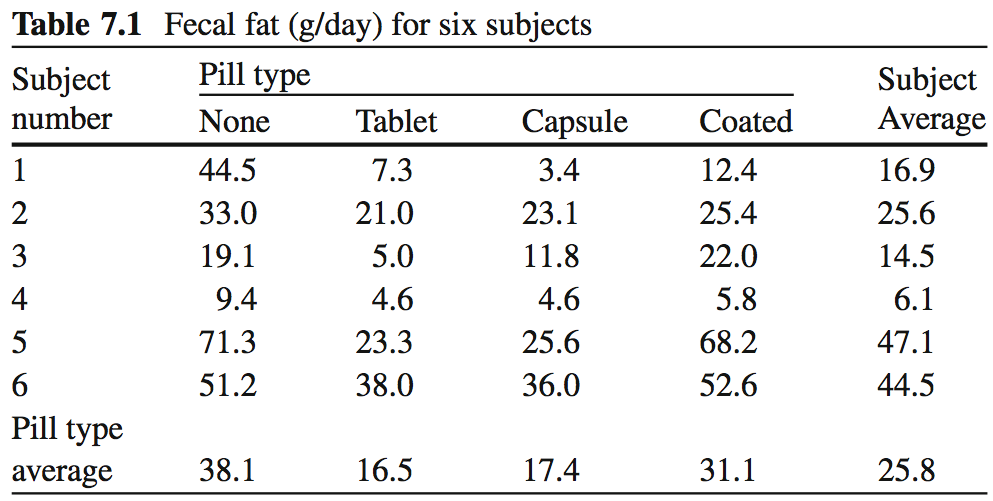
\includegraphics{VittinghoffTable71.png}
\caption{Fecal Fat dataset}
\end{figure}

\end{frame}

\begin{frame}{Fecal fat dataset}
\protect\hypertarget{fecal-fat-dataset-1}{}

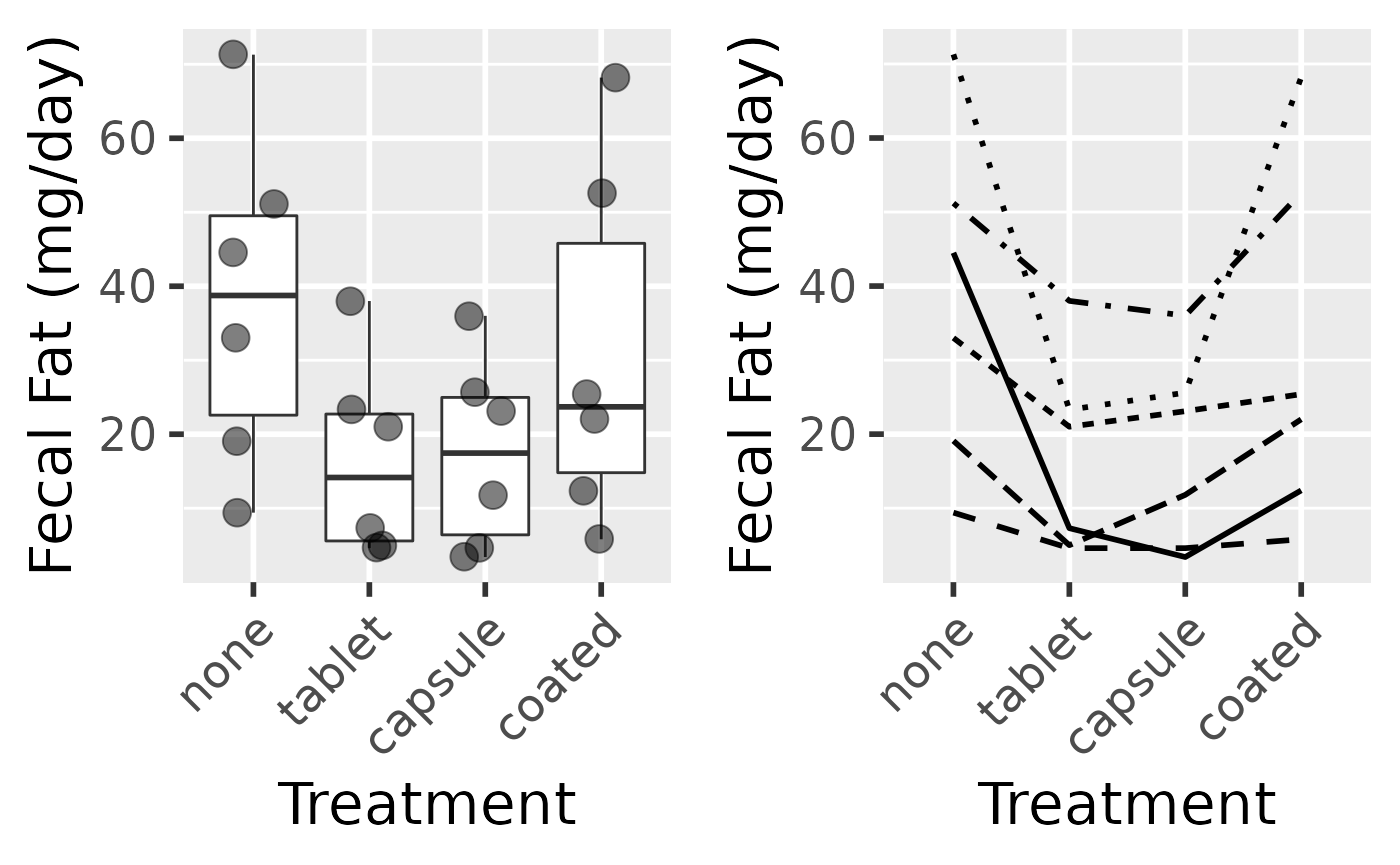
\includegraphics{../docs/articles/session_lecture_files/figure-beamer/boxplot-1.pdf}

\end{frame}

\begin{frame}{Analysis strategies for hierarchical data}
\protect\hypertarget{analysis-strategies-for-hierarchical-data}{}

\begin{itemize}
\tightlist
\item
  Fixed effects and other non-hierarchical strategies
\item
  Random / mixed effects models

  \begin{itemize}
  \tightlist
  \item
    model certain regression coefficients (intercept, slopes) as random
    variables
  \end{itemize}
\item
  Population average models

  \begin{itemize}
  \tightlist
  \item
    using Generalized Estimating Equations (GEE)
  \end{itemize}
\end{itemize}

\end{frame}

\hypertarget{non-hierarchical-analysis-strategies}{%
\section{Non-hierarchical analysis
strategies}\label{non-hierarchical-analysis-strategies}}

\begin{frame}{Non-hierarchical analysis strategies for hierarchical
data}
\protect\hypertarget{non-hierarchical-analysis-strategies-for-hierarchical-data}{}

\begin{itemize}
\tightlist
\item
  Analyses for each subgroup

  \begin{itemize}
  \tightlist
  \item
    e.g., look at each patient independently
  \item
    doesn't work at all in this example, and in general is not an
    integrated analysis of the whole data
  \item
    could sort of work for an example with many patients per doctor, a
    few doctors
  \end{itemize}
\item
  Analysis at the highest level in the hierarchy

  \begin{itemize}
  \tightlist
  \item
    first summarize data to highest level
  \item
    doesn't work at all in this example
  \item
    could sort of work for an example with few patients per doctor, many
    doctors
  \end{itemize}
\item
  Analysis on ``Derived Variables''

  \begin{itemize}
  \tightlist
  \item
    consider each treatment type separately, take differences in fat
    levels between treatment/control for each patient and use paired
    t-tests
  \item
    can work, but not for unbalanced groups
  \end{itemize}
\item
  Fixed-effects models
\end{itemize}

\end{frame}

\begin{frame}{When is hierarchical analysis definitely needed?}
\protect\hypertarget{when-is-hierarchical-analysis-definitely-needed}{}

\begin{enumerate}
\tightlist
\item
  the correlation structure is of interest, \emph{e.g.} familial
  aggregation of disease, or consistency of treatment within centers
\item
  we wish to ``borrow strength'' across the levels of a hierarchy in
  order to improve estimates
\item
  dealing with unbalanced data
\item
  we want to benefit from software designed for hierarchical data
\end{enumerate}

\end{frame}

\hypertarget{mixed-effects-models}{%
\section{Mixed effects models}\label{mixed-effects-models}}

\begin{frame}{Mixed effects models}
\protect\hypertarget{mixed-effects-models-1}{}

\begin{itemize}
\tightlist
\item
  Model looks like two-way ANOVA: \[
  FECFAT_{ij} = \beta_0 + \beta_{subject i} SUBJECT_i + \beta_{pilltype j} PILLTYPE_j + \epsilon_{ij}
  \]

  \begin{itemize}
  \tightlist
  \item
    Assumption:
    \(\epsilon_i \stackrel{iid}{\sim} N(0, \sigma_\epsilon^2)\)
  \end{itemize}
\item
  But instead of fitting a \(\beta\) to each individual, we assume that
  the subject effects are selected from a distribution of possible
  subject effects: \[
  FECFAT_{ij} = \beta_0 + SUBJECT_i + \beta_{pilltype j} PILLTYPE_j + \epsilon_{ij}
  \]
\end{itemize}

Where we assume: \(SUBJECT_i \stackrel{iid}{\sim} N(0, \tau_{00}^2)\)

\begin{itemize}
\tightlist
\item
  This is a \emph{mixed effects} model because:

  \begin{itemize}
  \tightlist
  \item
    the ``true'' intercept varies randomly from patient to patient
  \item
    the ``true'' (population) coefficient of treatment is fixed (the
    same for everyone)
  \end{itemize}
\end{itemize}

\end{frame}

\begin{frame}[fragile]{Fit this mixed-effects model}
\protect\hypertarget{fit-this-mixed-effects-model}{}

\begin{Shaded}
\begin{Highlighting}[]
\KeywordTok{library}\NormalTok{(nlme)}
\NormalTok{fitmix <-}\StringTok{ }\NormalTok{nlme}\OperatorTok{::}\KeywordTok{lme}\NormalTok{(fecfat }\OperatorTok{~}\StringTok{ }\NormalTok{pilltype, }
                    \DataTypeTok{data =}\NormalTok{ dat, }
                    \DataTypeTok{random =}  \OperatorTok{~}\StringTok{ }\DecValTok{1} \OperatorTok{|}\StringTok{ }\NormalTok{subject)}
\end{Highlighting}
\end{Shaded}

\tiny

Note: the \texttt{lme4} package is another popular alternative

\end{frame}

\begin{frame}[fragile]{Mixed effects model coeffients, variances, ICC}
\protect\hypertarget{mixed-effects-model-coeffients-variances-icc}{}

\tiny

\begin{verbatim}
## Linear mixed-effects model fit by REML
##   Data: dat 
##   Log-restricted-likelihood: -84.55594
##   Fixed: fecfat ~ pilltype 
##     (Intercept)  pilltypetablet pilltypecapsule  pilltypecoated 
##       38.083334      -21.550001      -20.666667       -7.016668 
## 
## Random effects:
##  Formula: ~1 | subject
##         (Intercept) Residual
## StdDev:    15.89557 10.34403
## 
## Number of Observations: 24
## Number of Groups: 6
\end{verbatim}

\(ICC = 15.9^2 / (15.9^2 + 10.34^2)\) = 0.7 = 0.7.

\normalsize

\begin{itemize}
\tightlist
\item
  Recall ICC is a measure of how large the subject effect is, in
  relation to the error term
\item
  Variances were estimated directly by the model!
\end{itemize}

\end{frame}

\begin{frame}{Assumptions of the mixed model}
\protect\hypertarget{assumptions-of-the-mixed-model}{}

\[
FECFAT_{ij} = \beta_0 + SUBJECT_i + \beta_{pilltype j} PILLTYPE_j + \epsilon_{ij}
\]

\begin{itemize}
\tightlist
\item
  Normally distributed residuals as in fixed effects model:

  \begin{itemize}
  \tightlist
  \item
    \(\epsilon_i \stackrel{iid}{\sim} N(0, \sigma_\epsilon^2)\)
  \end{itemize}
\item
  Normally distributed \textbf{latent variable}:

  \begin{itemize}
  \tightlist
  \item
    \(SUBJECT_i \stackrel{iid}{\sim} N(0, \tau_{00}^2)\)
  \end{itemize}
\end{itemize}

\end{frame}

\begin{frame}{Mixed effects model results}
\protect\hypertarget{mixed-effects-model-results}{}

A plot of the random intercept:
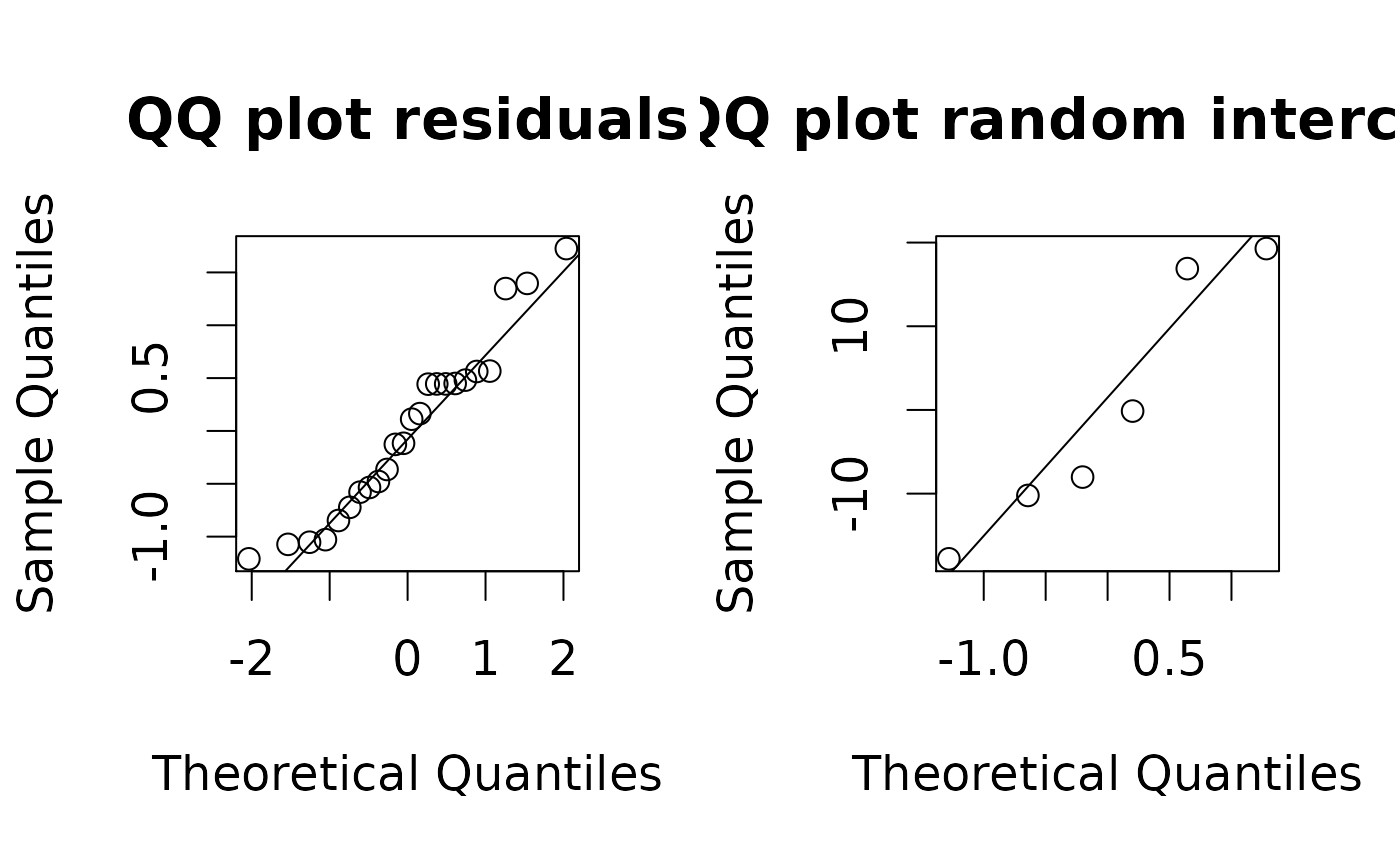
\includegraphics{../docs/articles/session_lecture_files/figure-beamer/unnamed-chunk-4-1.pdf}

\end{frame}

\begin{frame}{Mixed effects model diagnostics}
\protect\hypertarget{mixed-effects-model-diagnostics}{}

``
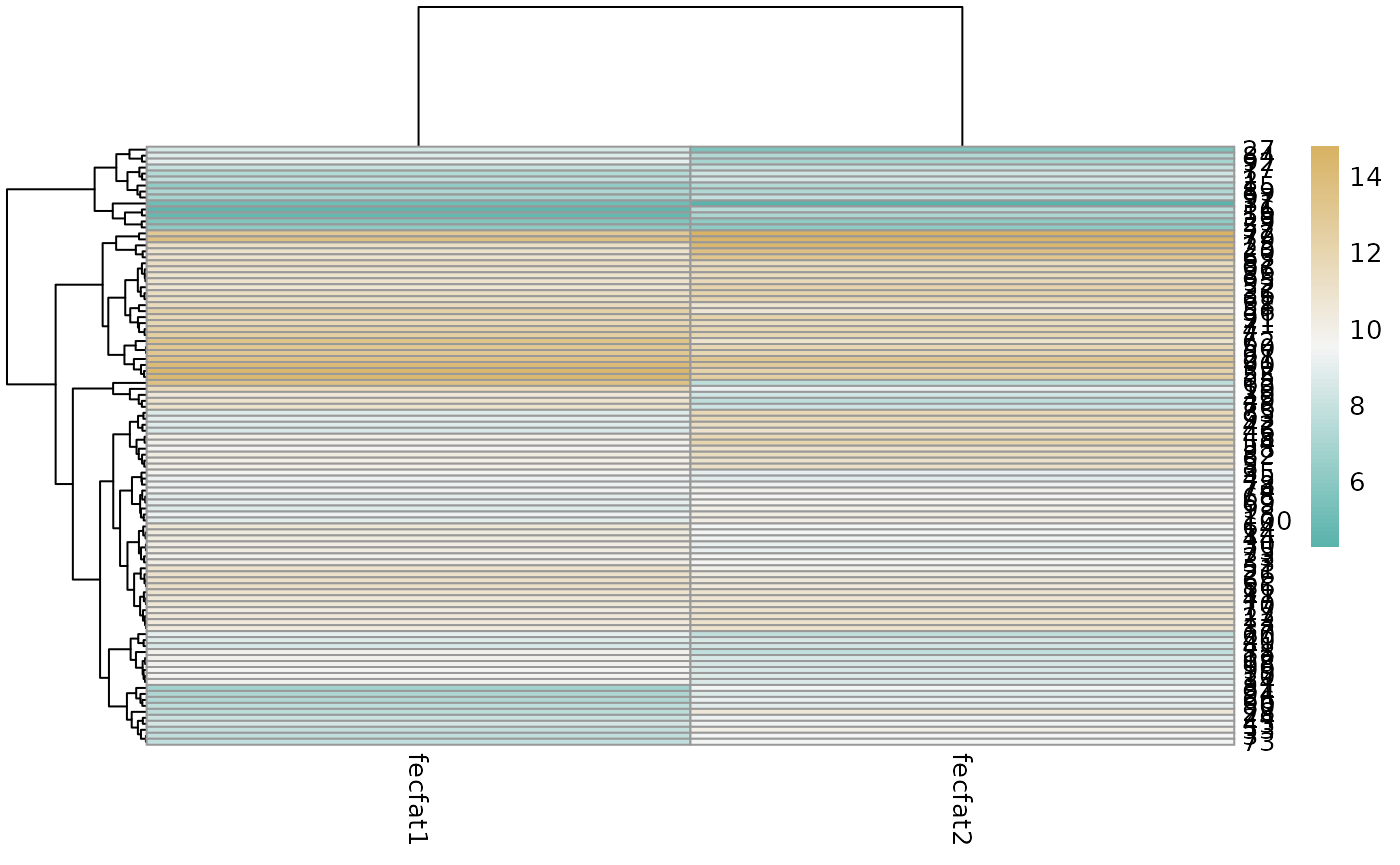
\includegraphics{../docs/articles/session_lecture_files/figure-beamer/unnamed-chunk-5-1.pdf}

\end{frame}

\begin{frame}[fragile]{Mixed effects model results}
\protect\hypertarget{mixed-effects-model-results-1}{}

\tiny

\begin{verbatim}
## Linear mixed-effects model fit by REML
##  Data: dat 
##        AIC      BIC    logLik
##   181.1119 187.0863 -84.55594
## 
## Random effects:
##  Formula: ~1 | subject
##         (Intercept) Residual
## StdDev:    15.89557 10.34403
## 
## Fixed effects: fecfat ~ pilltype 
##                     Value Std.Error DF   t-value p-value
## (Intercept)      38.08333  7.742396 15  4.918805  0.0002
## pilltypetablet  -21.55000  5.972127 15 -3.608430  0.0026
## pilltypecapsule -20.66667  5.972127 15 -3.460521  0.0035
## pilltypecoated   -7.01667  5.972127 15 -1.174903  0.2583
##  Correlation: 
##                 (Intr) plltypt plltypcp
## pilltypetablet  -0.386                 
## pilltypecapsule -0.386  0.500          
## pilltypecoated  -0.386  0.500   0.500  
## 
## Standardized Within-Group Residuals:
##          Min           Q1          Med           Q3          Max 
## -1.210052934 -0.615068039 -0.002727166  0.457105344  1.725618643 
## 
## Number of Observations: 24
## Number of Groups: 6
\end{verbatim}

\normalsize

\begin{itemize}
\tightlist
\item
  Note: correlation of the estimator of the fixed effects

  \begin{itemize}
  \tightlist
  \item
    high correlations may (but not necessarily) be due to collinearity
  \item
    not usually useful, not included in output of some packages
  \end{itemize}
\end{itemize}

\end{frame}

\begin{frame}[fragile]{Mixed effects model results}
\protect\hypertarget{mixed-effects-model-results-2}{}

Inference for variance terms (and fixed effects): \tiny

\begin{verbatim}
## Approximate 95% confidence intervals
## 
##  Fixed effects:
##                     lower       est.     upper
## (Intercept)      21.58081  38.083334 54.585860
## pilltypetablet  -34.27929 -21.550001 -8.820714
## pilltypecapsule -33.39595 -20.666667 -7.937381
## pilltypecoated  -19.74595  -7.016668  5.712618
## attr(,"label")
## [1] "Fixed effects:"
## 
##  Random Effects:
##   Level: subject 
##                   lower     est.    upper
## sd((Intercept)) 8.00117 15.89557 31.57904
## 
##  Within-group standard error:
##    lower     est.    upper 
##  7.23240 10.34403 14.79438
\end{verbatim}

\normalsize

\begin{itemize}
\tightlist
\item
  Would conclude that variation of the intercept between subjects is
  non-zero

  \begin{itemize}
  \tightlist
  \item
    not attributable to within-subject variation
  \end{itemize}
\end{itemize}

\end{frame}

\hypertarget{longitudinal-data}{%
\section{Longitudinal data}\label{longitudinal-data}}

\begin{frame}{Longitudinal data}
\protect\hypertarget{longitudinal-data-1}{}

\begin{itemize}
\tightlist
\item
  Interested in the change in the value of a variable within a
  ``subject''
\item
  Collect data repeatedly through time.
\item
  For hierarchical longitudinal analysis to be effective, before/after
  measurements need to be positively correlated
\end{itemize}

\end{frame}

\begin{frame}{Longitudinal data}
\protect\hypertarget{longitudinal-data-2}{}

\begin{itemize}
\tightlist
\item
  Interested in the change in the value of a variable within a
  ``subject''
\item
  Collect data repeatedly through time.
\item
  For hierarchical longitudinal analysis to be effective, before/after
  measurements need to be positively correlated
\end{itemize}

\end{frame}

\begin{frame}{Longitudinal data examples}
\protect\hypertarget{longitudinal-data-examples}{}

\begin{itemize}
\tightlist
\item
  Example 1: a measure of sleepiness before and after administration of
  treatment or placebo
\item
  Example 2: Study of Osteoporotic Fractores (SOF dataset)

  \begin{itemize}
  \tightlist
  \item
    9,704 women tracked with clinical visits every two years
  \item
    Bone Mineral Density (BMD), Body Mass Index (BMI), many other
    variables
  \end{itemize}
\item
  Questions for Example 2:

  \begin{enumerate}
  \tightlist
  \item
    Is change in BMD related to age at menopause? This is a
    time-invariant predictor, age at menopause, with time-dependent
    changes in the outcome, BMD.
  \item
    Is change in BMD related to change in BMI? This is an analysis
    relating a time-varying predictor, BMI, with changes in the outcome,
    BMD. BMI varies quite a lot between women, but also varies within a
    woman over time.
  \end{enumerate}
\end{itemize}

\end{frame}

\begin{frame}{Longitudinal data examples}
\protect\hypertarget{longitudinal-data-examples-1}{}

\begin{itemize}
\tightlist
\item
  birthweight and birth order
\item
  provides birthweights and order of infants from mothers who had 5
  children in Georgia

  \begin{itemize}
  \tightlist
  \item
    interested in whether birthweight of babies changes with order
  \item
    whether this difference depends on the \emph{mother's age at first
    childbirth} or on the \emph{weight of initial baby}.
  \end{itemize}
\end{itemize}

\end{frame}

\begin{frame}{Georgia Birthweights dataset}
\protect\hypertarget{georgia-birthweights-dataset}{}

Boxplot and ``Spaghetti'' plot:
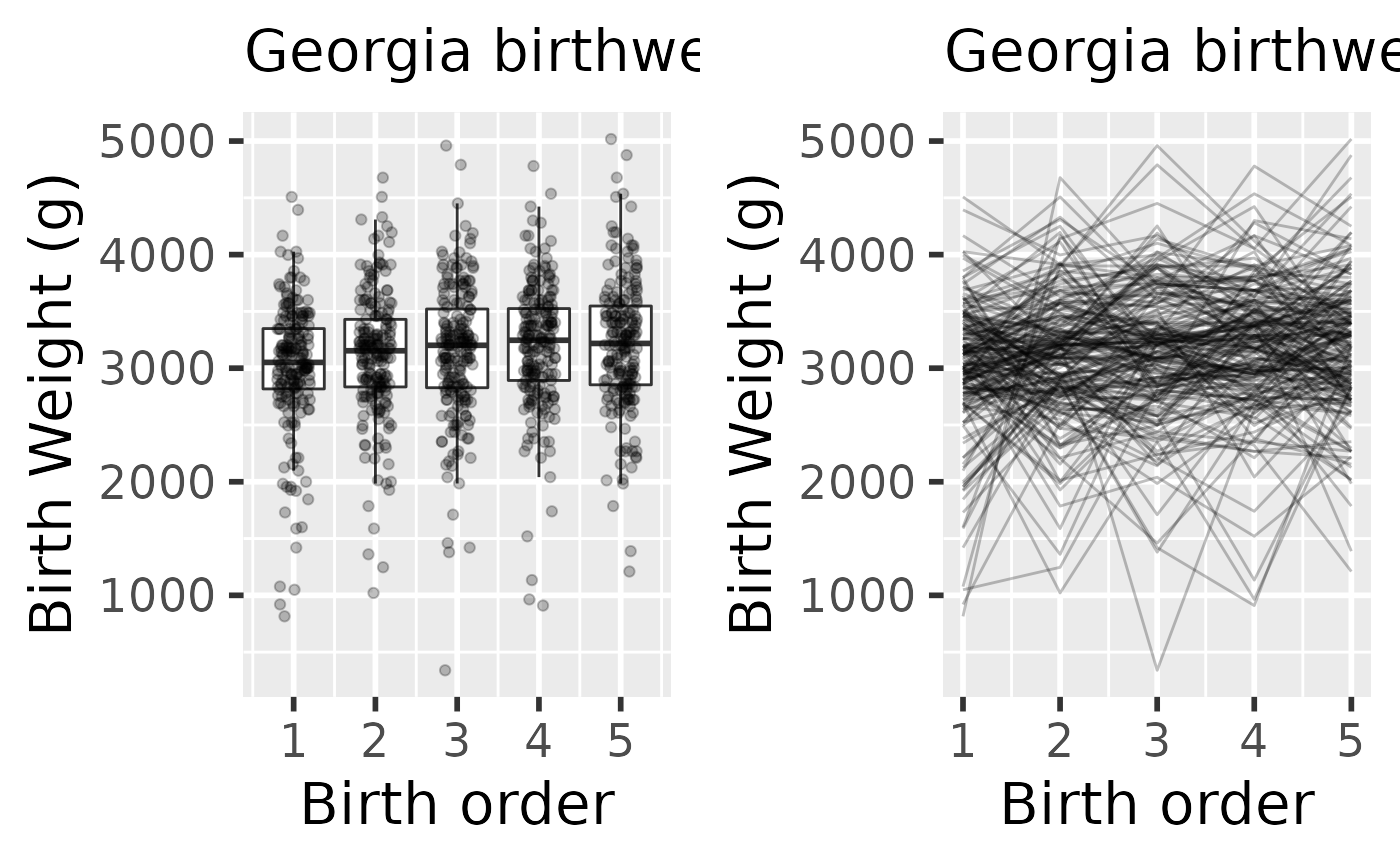
\includegraphics{../docs/articles/session_lecture_files/figure-beamer/unnamed-chunk-10-1.pdf}

\end{frame}

\begin{frame}[fragile]{Georgia Birthweights dataset}
\protect\hypertarget{georgia-birthweights-dataset-1}{}

\begin{itemize}
\tightlist
\item
  Does baseline birth weight vary by mother?

  \begin{itemize}
  \tightlist
  \item
    random intercept
  \end{itemize}
\end{itemize}

\begin{Shaded}
\begin{Highlighting}[]
\KeywordTok{library}\NormalTok{(nlme)}
\NormalTok{gafit1 <-}\StringTok{ }\KeywordTok{lme}\NormalTok{(bweight }\OperatorTok{~}\StringTok{ }\NormalTok{birthord, }\DataTypeTok{data=}\NormalTok{ga, }
              \DataTypeTok{random=}\OperatorTok{~}\DecValTok{1}\OperatorTok{|}\NormalTok{momid)}
\end{Highlighting}
\end{Shaded}

Note: there are not enough degrees of freedom to also fit a random
coefficient for birth order

\end{frame}

\begin{frame}{Georgia Birthweights dataset}
\protect\hypertarget{georgia-birthweights-dataset-2}{}

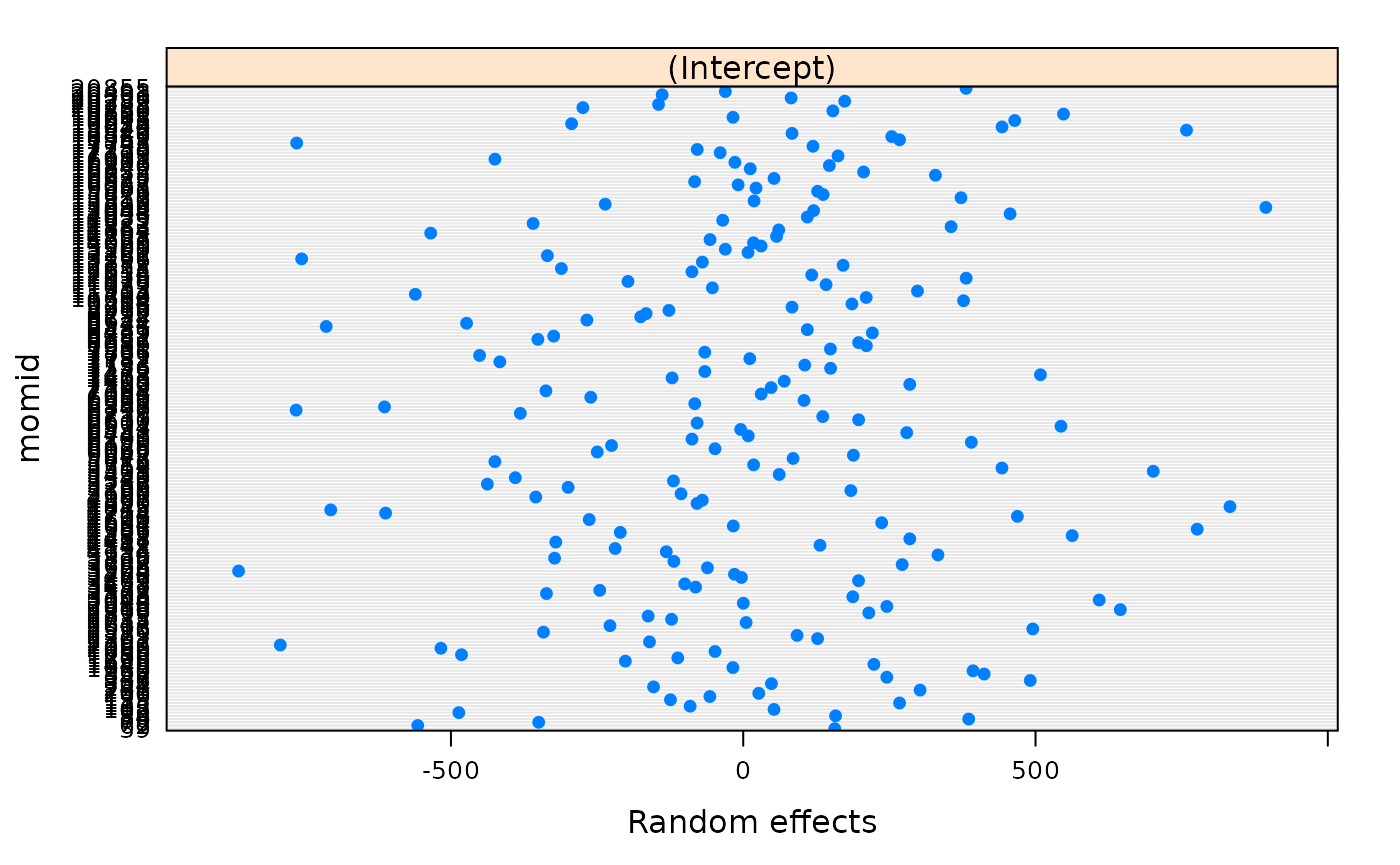
\includegraphics{../docs/articles/session_lecture_files/figure-beamer/unnamed-chunk-12-1.pdf}

\end{frame}

\begin{frame}[fragile]{Georgia Birthweights dataset}
\protect\hypertarget{georgia-birthweights-dataset-3}{}

\tiny

\begin{Shaded}
\begin{Highlighting}[]
\KeywordTok{summary}\NormalTok{(gafit1)}
\end{Highlighting}
\end{Shaded}

\begin{verbatim}
## Linear mixed-effects model fit by REML
##  Data: ga 
##        AIC      BIC    logLik
##   15321.65 15341.28 -7656.826
## 
## Random effects:
##  Formula: ~1 | momid
##         (Intercept) Residual
## StdDev:    367.2676 445.0228
## 
## Fixed effects: bweight ~ birthord 
##                Value Std.Error  DF  t-value p-value
## (Intercept) 2995.640  41.99615 799 71.33130       0
## birthord      46.608   9.95101 799  4.68374       0
##  Correlation: 
##          (Intr)
## birthord -0.711
## 
## Standardized Within-Group Residuals:
##         Min          Q1         Med          Q3         Max 
## -5.26801358 -0.43683345  0.05028638  0.52703429  3.30770805 
## 
## Number of Observations: 1000
## Number of Groups: 200
\end{verbatim}

\end{frame}

\begin{frame}[fragile]{Georgia Birthweights dataset}
\protect\hypertarget{georgia-birthweights-dataset-4}{}

\tiny

\begin{Shaded}
\begin{Highlighting}[]
\KeywordTok{intervals}\NormalTok{(gafit1, }\DataTypeTok{which =} \StringTok{"all"}\NormalTok{)}
\end{Highlighting}
\end{Shaded}

\begin{verbatim}
## Approximate 95% confidence intervals
## 
##  Fixed effects:
##                  lower     est.      upper
## (Intercept) 2913.20418 2995.640 3078.07582
## birthord      27.07478   46.608   66.14122
## attr(,"label")
## [1] "Fixed effects:"
## 
##  Random Effects:
##   Level: momid 
##                    lower     est.    upper
## sd((Intercept)) 323.1724 367.2676 417.3794
## 
##  Within-group standard error:
##    lower     est.    upper 
## 423.7298 445.0228 467.3859
\end{verbatim}

\normalsize

\begin{itemize}
\tightlist
\item
  Do birth weights or the effect of birth order vary by mother?

  \begin{itemize}
  \tightlist
  \item
    yes: both standard deviations are non-zero
  \end{itemize}
\end{itemize}

\end{frame}

\hypertarget{population-average-models}{%
\section{Population Average Models}\label{population-average-models}}

\begin{frame}{Population Average Models}
\protect\hypertarget{population-average-models-1}{}

\begin{itemize}
\tightlist
\item
  An alternative to random / mixed-effects models that is more robust to
  assumptions of:

  \begin{itemize}
  \tightlist
  \item
    distribution of random effects
  \item
    correlation structure
  \end{itemize}
\item
  Estimates correlation structure from the data rather than assuming
  normality

  \begin{itemize}
  \tightlist
  \item
    Requires more clusters than observations per cluster
  \end{itemize}
\item
  Estimates regression coefficients and robust standard errors

  \begin{itemize}
  \tightlist
  \item
    commonly by Generalized Estimating Equations (GEE)
  \end{itemize}
\end{itemize}

\end{frame}

\begin{frame}{Population Average Models}
\protect\hypertarget{population-average-models-2}{}

\begin{itemize}
\item
  Compare mixed model multiple linear regression: \[
  E[Y_{ij}|X_{ij}] = \beta_0 + \alpha_{0j} + \beta_1 X_{ij}, \alpha_{0j} \sim N(0, \sigma)
  \] for subject \(i\) in group \(j\).
\item
  to a population average model: \[
  E[Y_{ij}|X_{ij}] = \beta_0^* + \beta_1^* X_{ij}
  \]
\item
  Interpretations of \(\beta^*\) and \(\beta\) are equivalent
\item
  Numerically equivalent for linear and log-linear models (if
  specification of mixed model is correct), but not for logistic link.
\end{itemize}

\end{frame}

\begin{frame}[fragile]{Fit a population average model}
\protect\hypertarget{fit-a-population-average-model}{}

\begin{Shaded}
\begin{Highlighting}[]
\NormalTok{gafit.gee <-}\StringTok{ }\NormalTok{gee}\OperatorTok{::}\KeywordTok{gee}\NormalTok{(bweight }\OperatorTok{~}\StringTok{ }\NormalTok{birthord,}
                      \DataTypeTok{corstr =} \StringTok{"exchangeable"}\NormalTok{,}
                      \DataTypeTok{id =}\NormalTok{ momid,}
                      \DataTypeTok{data =}\NormalTok{ ga)}
\end{Highlighting}
\end{Shaded}

\end{frame}

\begin{frame}[fragile]{}
\protect\hypertarget{section}{}

\tiny

\begin{Shaded}
\begin{Highlighting}[]
\KeywordTok{summary}\NormalTok{(gafit.gee)}
\end{Highlighting}
\end{Shaded}

\begin{verbatim}
## 
##  GEE:  GENERALIZED LINEAR MODELS FOR DEPENDENT DATA
##  gee S-function, version 4.13 modified 98/01/27 (1998) 
## 
## Model:
##  Link:                      Identity 
##  Variance to Mean Relation: Gaussian 
##  Correlation Structure:     Exchangeable 
## 
## Call:
## gee::gee(formula = bweight ~ birthord, id = momid, data = ga, 
##     corstr = "exchangeable")
## 
## Summary of Residuals:
##       Min        1Q    Median        3Q       Max 
## -2795.464  -299.126    48.840   341.144  1824.536 
## 
## 
## Coefficients:
##             Estimate Naive S.E.   Naive z Robust S.E.  Robust z
## (Intercept) 2995.640  41.973695 71.369462   38.808066 77.191170
## birthord      46.608   9.958128  4.680398    9.996256  4.662546
## 
## Estimated Scale Parameter:  332525.3
## Number of Iterations:  1
## 
## Working Correlation
##           [,1]      [,2]      [,3]      [,4]      [,5]
## [1,] 1.0000000 0.4035684 0.4035684 0.4035684 0.4035684
## [2,] 0.4035684 1.0000000 0.4035684 0.4035684 0.4035684
## [3,] 0.4035684 0.4035684 1.0000000 0.4035684 0.4035684
## [4,] 0.4035684 0.4035684 0.4035684 1.0000000 0.4035684
## [5,] 0.4035684 0.4035684 0.4035684 0.4035684 1.0000000
\end{verbatim}

\end{frame}

\begin{frame}{Correlation assumptions for GEE}
\protect\hypertarget{correlation-assumptions-for-gee}{}

Must make some assumption about the form of correlation among grouped
observations. Some options are:

\begin{itemize}
\tightlist
\item
  Independence:

  \begin{itemize}
  \tightlist
  \item
    no correlation between measurements within group
  \end{itemize}
\item
  Exchangeable:

  \begin{itemize}
  \tightlist
  \item
    all pairwise correlations are the same (in large-N limit)
  \item
    nothing distinguishes one member of a cluster from another
  \item
    appropriate in the absence of other data structures such as
    measurements taken through time or space
  \end{itemize}
\item
  Auto-regressive (\emph{AR-M}):

  \begin{itemize}
  \tightlist
  \item
    observations taken more closely in time are more highly correlated
  \end{itemize}
\end{itemize}

\end{frame}

\begin{frame}{Correlation assumptions for GEE (cont'd)}
\protect\hypertarget{correlation-assumptions-for-gee-contd}{}

\begin{itemize}
\tightlist
\item
  Unstructured:

  \begin{itemize}
  \tightlist
  \item
    estimates a separate correlation between observations taken on each
    pair of ``times''
  \end{itemize}
\item
  Non-stationary (``non\_stat\_M\_dep''):

  \begin{itemize}
  \tightlist
  \item
    similar to unstructured, but assumes all correlations for pairs
    separated far enough in time are zero
  \end{itemize}
\item
  Stationary (``stat\_M\_dep''):

  \begin{itemize}
  \tightlist
  \item
    e.g.~stationary of order 2: observations taken at time points 1 and
    3 have the same correlation as time points 2 and 4
  \item
    but this might be different from the correlation between
    observations taken at times 2 and 3
  \item
    correlations for observations 3 or more time periods apart assumed
    to be zero
  \end{itemize}
\end{itemize}

\emph{Fewer assumptions requires more data, and good assumptions improve
results}

\end{frame}

\begin{frame}{Help in choosing a method}
\protect\hypertarget{help-in-choosing-a-method}{}

\begin{figure}
\centering
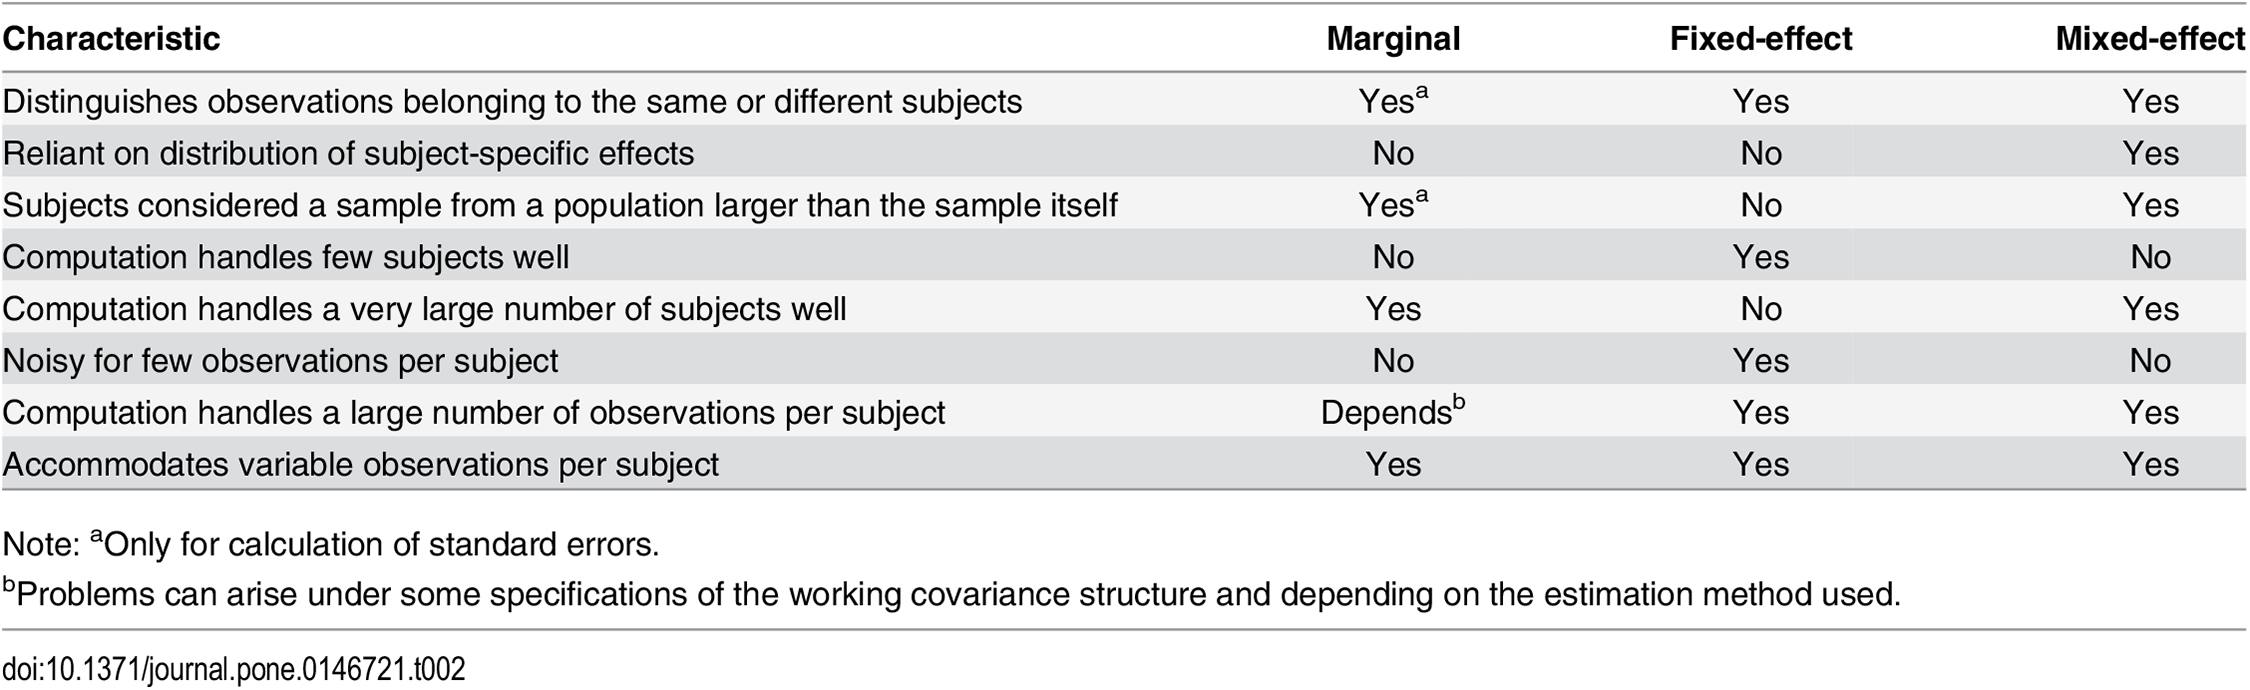
\includegraphics{journal.pone.0146721.t002.PNG}
\caption{Hierarchical modeling decision table from Moen \emph{et al.}}
\end{figure}

\end{frame}

\begin{frame}{Conclusions}
\protect\hypertarget{conclusions}{}

\begin{itemize}
\tightlist
\item
  Ignoring within-subject correlations can produce very wrong results,
  and is not always ``conservative''
\item
  Hierarchical analysis strategies are needed for any of:

  \begin{enumerate}
  \tightlist
  \item
    When the correlation structure is of primary interest, \emph{e.g.}
    familial aggregation of disease, or consistency of treatment within
    centers,
  \item
    When we wish to ``borrow strength'' across the levels of a hierarchy
    in order to improve estimates, and
  \item
    When dealing with unbalanced correlated data. E.g., no requirement
    that each Georgia mother have exactly 5 children.
  \end{enumerate}
\item
  Population average models provide a robust alternative to mixed models

  \begin{itemize}
  \tightlist
  \item
    for one level of hierarchy
  \end{itemize}
\end{itemize}

\end{frame}

\begin{frame}{A final note on reporting results of hypothesis tests}
\protect\hypertarget{a-final-note-on-reporting-results-of-hypothesis-tests}{}

\begin{itemize}
\tightlist
\item
  Include test statistic, a measure of ``effect size'', and test name if
  unclear from test statistic
\item
  Write in plain language and let the statistics support, not lead.
  E.g.:

  \begin{itemize}
  \tightlist
  \item
    \emph{do}: The 36 study participants had a mean age of 27.4 (SD =
    12.6), significantly older than the university mean of 21.2 years
    (t(35) = 2.95, p = 0.01).
  \item
    \emph{don't}: A p-value of 0.01 indicated significant difference in
    age of study participants compared to all university students.
  \item
    \emph{do}: report confidence intervals where possible
  \end{itemize}
\end{itemize}

\tiny

\begin{itemize}
\tightlist
\item
  \href{https://psych.uw.edu/storage/writing_center/stats.pdf}{UW
  ``Reporting Results of Common Statistical Tests in APA Format''}:
  specific examples of reporting a hypothesis test result
\item
  STROBE guidelines for reporting observational studies:
  \url{https://www.strobe-statement.org/}
\item
  \href{https://academic.oup.com/DocumentLibrary/JJCO/eng.guideline.pdf}{A
  Guideline for Reporting Results of Statistical Analysis in Japanese
  Journal of Clinical Oncology}: helpful guidelines for all parts of a
  manuscript
\end{itemize}

\end{frame}

\begin{frame}{CONGRATULATIONS!!!}
\protect\hypertarget{congratulations}{}

\end{frame}

\end{document}
